\documentclass{article}

\usepackage{xcolor}
\usepackage{tcolorbox}     % Color boxes
\usepackage{amsmath}       % Basic mathematical typesetting
\usepackage{amssymb}       % Advanced math symbols
\usepackage{amsthm}        % Theorems typesetting
\usepackage{array}         % Advanced table column formats
\usepackage{enumitem}      % Itemize/enumrate
\usepackage{fancyhdr}      % Custom header/footer styles
\usepackage{fourier}       % Adobe Utopia font
\usepackage{graphicx}      % Enhanced images support
\usepackage{ifluatex}      % LuaTeX-specific options
\usepackage{kantlipsum}    % English kantian-style lipsum
\usepackage{lipsum}        % Lorem ipsum
\usepackage{listings}      % Code listings
\usepackage{longtable}     % Multi-page tables
\usepackage{multirow}      % Advanced table cells
\usepackage{setspace}      % Set space between lines
\usepackage{scrextend}     % Allows \addmargin environment
\usepackage{tablefootnote} % Table footnotes
\usepackage{tocloft}       % Custom ToC/LoF/LoT
\usepackage{url}           % URL-sensitive line breaks
\usepackage{xspace}        % Remove duplicated spaces
\usepackage{tabularx}

\setstretch{1.15}
\setlength{\parindent}{5mm}
\counterwithin{equation}{section}
\counterwithin{figure}{section}
\counterwithin{table}{section}
\setcounter{tocdepth}{3}
\setcounter{secnumdepth}{3}

% List formatting
\setlist[itemize,1]{topsep=2pt,label=\large$\bullet$, leftmargin=28pt}
\setlist[itemize,2]{topsep=2pt,leftmargin=18pt}
\setlist[itemize,3]{topsep=2pt,leftmargin=18pt}
\setlist[enumerate,1]{topsep=2pt,leftmargin=24pt}
\setlist[enumerate,2]{topsep=2pt,leftmargin=16pt}
\setlist[enumerate,3]{topsep=2pt,leftmargin=16pt}

% TabularX columns
\newcolumntype{R}{>{\raggedleft\arraybackslash}X}

% region LuaLatex Scripts

% Script from: https://github.com/ArturB/WUT-Thesis
\usepackage{ifluatex}      % LuaTeX-specific options
\ifluatex
    \usepackage[T1]{fontenc}
    \usepackage[utf8]{luainputenc}
    \usepackage{luacode}
    % In LuaTeX, we can prevent one-letter words
    % from beging at the end of the line.
    \begin{luacode}
    local debug = false
    local glyph_id = node.id "glyph"
    local glue_id  = node.id "glue"
    local hlist_id = node.id "hlist"

    local prevent_single_letter = function (head)
        while head do
            if head.id == glyph_id then
                if unicode.utf8.match(unicode.utf8.char(head.char),"%a") then     -- is a letter
                    if head.prev.id == glue_id and head.next.id == glue_id then   -- is one letter word

                        local p = node.new("penalty")
                        p.penalty = 10000

                        if debug then
                            local w = node.new("whatsit","pdf_literal")
                            w.data = "q 1 0 1 RG 1 0 1 rg 0 0 m 0 5 l 2 5 l 2 0 l b Q"
                            node.insert_after(head,head,w)
                            node.insert_after(head,w,p)
                        else
                            node.insert_after(head,head,p)
                        end
                    end
                end
            end
            head = head.next
        end
        return true
    end

    luatexbase.add_to_callback("pre_linebreak_filter",prevent_single_letter,"~")
    \end{luacode}
\fi

% endregion

% region Custom Tags

\newcommand{\temporary}[1]{
    \begin{tcolorbox}[colframe=red, colback=white, title={\textbf{WERSJA PO POLSKU}}, sharp corners=south]
        #1
    \end{tcolorbox}
}

% endregion

\begin{document}
    % List of figures
    \renewcommand*\l@figure{\@dottedtocline{1}{0.5em}{2.25em}}
    \newcommand{\listoffigurestoc}{
        \listoffigures
        \addcontentsline{toc}{section}{\listfigurename}
    }

    % List of tables
    \renewcommand*\l@table{\@dottedtocline{1}{0.5em}{2.25em}}
    \newcommand{\listoftablestoc}{
        \listoftables
        \addcontentsline{toc}{section}{\listtablename}
    }

    \title{Title of article}
    \author{Patryk Filip Gryz}

    \maketitle

    \clearpage
    \section{Introduction}

        \subsection{Background}

            The discovery of DNA marked the beginning of a new era in biology and medicine, enabling research into the molecular foundations of life and the precise diagnosis of many diseases\cite{Louie:2000}. In 1953, the structure of the DNA double helix was discovered by Watson and Crick\cite{Watson:1953}. In 1970, Francis Crick formulated the central dogma of molecular biology\cite{Crick:1970}, which states that genetic information flows from DNA to RNA and then to proteins, forming the foundation of modern molecular biology. In 1977, the complete genetic material of the DNA virus — bacteriophage $\phi{}$X174 was sequenced\cite{Sanger:1977:2}. This discovery highlighted the limitations of traditional analysis methods and demonstrated the need for computers to process DNA sequences\cite{Staden:1979}. In the 1980s, the European "EBML Data Library" was funded\cite{Higgins:1992}, and in 1982, the United States launched "GenBank"\cite{Bilofsky:1986}. In 1998, Jo Handelsman proposed the analysis of genetic material from many organisms simultaneously, without the need for cultivation, with his team studying organisms present in soil\cite{Handelsman:1998}. The use of information about genetic material found in the environment, combined with sequence databases, enables the identification of organisms present in a given sample. However, the process of analyzing large numbers of DNA sequences and comparing them to databases requires significant computational resources. With the development of next-generation sequencing methods\cite{Reinartz:2002}, sequencing costs have decreased significantly, and the number of DNA sequences being analyzed has increased\cite{Muir:2016}. Further accumulation of sequence data and increasing sequencing throughput lead to a growing demand for computational resources.
        
        \subsection{Motivation}

            The time required for taxonomic classification of large sequence datasets using traditional tools, such as BLAST, can span several hours, even for relatively small collections of sequences e.g. 4096 sequences. In many fields, artificial neural networks (ANN) have demonstrated the ability to outperform classical heuristic algorithms, offering faster and more accurate results. By leveraging the capabilities of ANN, this works aims to accelerate taxonomic clasisfication process while maintaining at least the same level of quality as traditional methods.

        \subsection{Objectives}
    
            The primary objective of this study is to leverage an artificial neural network to support the selection of representative genetic sequences for taxonomic classification. Instead of classifying entire environmental genetic sequences sample, the proposed approach focuses on identifying a subset of sequences that best represent the sample. These selected representatives are then classified, reducing computational complexity while maintaining classification accuracy.

        \subsection{Main Contributions}

            This paper introduces a novel artificial neural network model for calculating dissimilarities between genetic sequences, which can be used in clustering algorithm to select representative sequences for taxonomic classification. We provide all the necessary components for training the model, including dataset preparation, batch process, a loss function, and a training loop. The paper also includes an application that can perform taxonomic classification with specified parameters. Furthermore, we develope a library that allows users to compose the taxonomic classification pipelines.

        \subsection{Structure of the Paper}

            The rest of the paper is organized as follows. Section 2 provides a description of related work, reviewing previous research on taxonomic classification and highlights a research gap. Section 3 defines the problem, presents the proposed approach, and provides detailed implementation details. Section 4 describes the experimental setup, including used datasets, the performance metrics for evaluation, and the results obtained from experiments with analysis. Section 5 interprets the results, discusses the limtiations of proposed approach, and explores possible improvements for future work. Finally, Section 6 concludes the paper by summarizing the main findings and suggesting potential directions for future research.

    \clearpage
    \section{Related Work}

        \subsection{Overview of Existing Approaches}

            \temporary{
                Badania nad klasyfikacją taksonomiczną sekwencji DNA cechują się dynamicznym rozwojem w ciągu ostatnich 25 lat. Wprowadzenie metod sekwencjonowania nowej generacji pozwoliło na analizę dużych ilości materiału genetycznego pochodzącego z różnych środowisk. Optymalizacja procesu klasyfikacji taksonomicznej stała się głównym kierunkiem rozwoju narzędzi do klasyfikacji, szczególnie w przypadku narzędzi opartych na bazach danych sekwencji genetycznych, ponieważ liczba sekwencji w tych bazach podwaja się średnio co 30 miesięcy~\cite{Benson:2008}.

        Historycznie jednym z pierwszych algorytmów, który umożliwił klasyfikację taksonomiczną był algorytm Needlemana-Wunscha\cite{Needleman:1970} opracowany w 1970 roku, który pozwalał na porównywanie sekwencji genetycznych. Jednak pierwszym rozwiązaniem, które pozwalało na klasyfikację taksonomiczną w rozsądnym czasie, było narzędzie stworzone w 1983 roku przez D. Lipmana i W. Wilbura\cite{Wilbur:1983}. Bazowało ono na podziale sekwencji na $k$-krotki, które są uogólnieniem $k$-merów i ich porównywaniu. Rozwinięciem tego rozwiązania był algorytm ,,BLAST'' przedstawiony w 1990 roku\cite{Altschul:1990} bazujący na $k$-merach oraz umożliwiający wyszukiwanie sekwencji podobnych w bazach NCBI. Innym podejściem powstałym w podobnym okresie było narzędzie ,,Clustal''\cite{Higgins:1988} stworzone w 1988 roku, które pozwalało na wyrównywanie wielu sekwencji genetycznych.

        Największy postęp w badaniach nastąpił jednak w ciągu ostatnich 15 lat, czego przykładem jest utworzenie w 2012 roku narzędzia ,,MetaPhlAn''\cite{Segata:2012}, które wykorzystuje geny wskaźnikowe do porównywania składu gatunkowego próbek metagenomicznych. Kolejnym podejściem opartym na genach wskaźnikowych jest narzędzie ,,mOTUs2''\cite{Milanese:2019}, które bazuje na identyfikacji i analizie markerów unikalnych dla specyficznych szczepów mikroorganizmów. Inne podejście zostało zastosowane w narzędziu ,,Centrifuge''\cite{Kim:2016} opracowanym w 2016 roku, które wykorzystuje indeksowanie sekwencji za pomocą transformacji Burrowsa-Wheelera\cite{Burrows:1994} oraz indeksu Ferraginy-Manziniego\cite{Ferragina:2000} w celu efektywne wyszukiwania sekwencji podobnych. Bardziej klasyczne podejście zostało zastosowane w narzędziu ,,Kraken''\cite{Wood:2014} przedstawionym w 2014 roku, które wykorzystuje $k$-mery wraz z indeksowaną bazą sekwencji.

        Inną metodę optymalizacji procesu klasyfikacji taksonomicznej przedstawili Gautier i Lund w 2013 roku\cite{Gautier:2013}. Ich metoda opierała się na rozproszonej architekturze, w której serwer zwracał wskazówki dotyczące możliwych sekwencji do analizy na podstawie losowo wybranych sekwencji wejściowych, co pozwoliło na redukcję przesyłanych danych przez sieć. Nietypowe podejście do zadania klasyfikacji taksonomicznej przedstawiono w 2022 roku w narzędziu ,,BERTax''\cite{Mock:2022}. Narzędzie to wykorzystuje model typu transformer\cite{Transformers} do analizy sekwencji DNA, traktując je jako specyficzny język, na podstawie którego można dokonać przypisania bez potrzeby korzystania z baz referencyjnych. Kolejnym rozwiązaniem wykorzystującym modele uczenia maszynowego jest narzędzie ,,CGRclust''\cite{Alipour:2024}, które grupuje sekwencje DNA za pomocą dwuwymiarowej reprezentacji gier chaosu, łącząc nienadzorowane uczenie kontrastowe ze splotowymi sieciami neuronowymi.
            }

        \subsection{Comparatie Analysis}

            \temporary{
                Algorytmy bazujące na jakości wyrównania dają dobre wyniki, ale działają bardzo wolno.
                Algorytmy bazujące na $k$-merach działają szybko, ale nie uwzgledniają ukrytych wzorów w sekwencjach genetycznych
            }

        \subsection{Research Gaps}

            \temporary{
                Choć w ostatnich latach pojawiły się badania dotyczące klasyfikacji taksonomicznej z wykorzystaniem metod uczenia maszynowego, to wciąż brakuje prac skupiających się na zastosowaniu sztucznych sieci neuronowych z uczeniem kontrastowym do efektywnego grupowania sekwencji, co mogłoby znacząco przyspieszyć proces klasyfikacji przy użyciu dostępnych narzędzi.
            }

    \clearpage
    \section{Methodology}

        \subsection{Problem Definition}

            \temporary{
                Klasyfikacja taksonomiczna:

                Dla zbioru sekwencji A, szukamy takiego zbioru organizmów, że 

                \[
                    \forall a \in A \exists b \in B \text{ takie, że } a \text{ jest lokalnie podobne do } b_{sequence}
                \]
            }

        \subsection{Proposed Approach / Algorithm / Model}

            \temporary{
                W pracy zostaną wykorzystane dwa klasyczne podejścia do klasyfikacji taksonomicznej sekwencji genetycznych. Pierwsze z nich opiera się na wyrównaniu sekwencji, przy czym zostanie wykorzystany zmodyfikowany algorytm Needlemana-Wunscha. Drugie podejście wykorzystuje $k$-mery, w którym do obliczeń zostana zastosowane proste zanurzenia oraz odległość euklidesowa.

                \subsubsection{Algorytm Needlemana-Wunscha}
        
                    Algorytm Needlemana-Wunscha jest klasycznym algorytmem do wyrównywania globalnego sekwencji genetycznych. Metoda ta polega na zbudowaniu macierzy podobieństwa między sekwencjami zgodnie z ustalonymi regułami, które zostały przedstawione w równaniu~\eqref{Equation:NeedlemanWunsch}. W przypadku klasyfikacji taksonomicznej do dalszych obliczeń wystarczy wartość jakości dopasowania zawarta w $D_{n + 1, m + 1}$.
        
                    \begin{equation}
                        \begin{aligned}
                            D_{i,0} &= i \cdot g, & \text{dla } & i \in [1, n + 1] \\
                            D_{0,j} &= j \cdot g, & \text{dla } & j \in [2, m + 1] \\
                            D_{i,j} &= \max
                            \begin{cases}
                                D_{i - 1, j} + g \\
                                D_{i, j - 1} + g \\
                                D_{i - 1, j - 1} + s(A_i, B_j)
                            \end{cases}, & \text{dla } & i \in (1, n + 1] \text{ oraz } j \in (1, m + 1]
                        \end{aligned}
                        \label{Equation:NeedlemanWunsch}
                    \end{equation}
        
                    gdzie:
                    \begin{align*}
                        A, B -& \text{porównywane sekwencje}, \\
                        n, m -& \text{długości sekwencji } A \text{ oraz } B, \\
                        D -& \text{macierz podobieństwa o rozmiarach } n + 1 \text{ x } m + 1, \\
                        g \in \mathbb{R} -& \text{kara za przerwę}, \\
                        s(A_i, B_j) \in \mathbb{R} -& \text{podobieństwo między } i \text{-tym elementem w sekwencji A,} \\
                        & \text{a } j \text{-tym elementem w sekwencji B}. \\
                    \end{align*}
        
                \subsubsection{Zanurzenia $k$-merów}
        
                    Wykorzystanie $k$-merów w roli zanurzeń pozwala na reprezentację sekwencji DNA w postaci wektorów liczbowych, które można porównywać za pomocą różnych miar, takich jak na przykład odległość euklidesowa. Wektory liczbowe pozwalają na kompaktową reprezentację długich sekwencji, co znacznie przyśpiesza procesy grupowania sekwencji oraz klasyfikacji taksonomicznej. Metoda ta jest obecnie jedną z najpopularniejszych metod stosowanych do klasyfikacji taksonomicznej z wykorzystaniem baz danych, ponieważ cechuje się wysoką prędkością działania oraz pozwala uzyskać dobre wyniki. Obecne narzędzia wykorzystują różne miary, parametry $k$ oraz dodatkowe mechanizmy do dalszej optymalizacji tej metody.

                    \subsubsection{Sztuczna sieć neuronowa}

            Nową zaproponowaną metodą jest wykorzystanie sztucznej sieci neuronowej do redukcji wymiarowości wejściowych sekwencji DNA do postaci wektora cech o wymiarze $\mathbb{R}^{64}$. Sztuczna sieć neuronowa wykorzystuje uczenie kontrastowe, które umożliwia naukę reprezentacji danych wejściowych z zachowaniem własności podobieństwa oraz niepodobieństwa między wejściowymi sekwencjami. Niepodobieństwo między sekwencjami zostanie obliczone poprzez obliczenie niepodobieństwa kosinusowego wyrażonego wzorem~\eqref{Equation:CosineDissimilarity} między wektorami cech sekwencji DNA.

            \paragraph{Architektura}
                Architektura modelu sztucznej sieci neuronowej składa się z dwóch bloków splotowych oraz bloku perceptronów wielowarstwowych. Każdy z bloków splotowych zawiera warstwę splotową oraz warstwę normalizacji wsadowej i jest odpowiedzialny za ekstrakcję niskopoziomowych cech sekwencji. Ostatni blok splotowy jest połączony z blokiem perceptronów wielowarstwowych za pomocą warstwy spłaszczającej. Blok perceptronów wielowarstwowych odpowiada za tworzenie reprezentacji sekwencji, składa się z trzech warstw, które wykorzystują funkcję aktywacji GELU\cite{Hendrycks:2016}, z wyjątkiem ostatniej warstwy. Wyjściem całego modelu jest wektor cech o wymiarze $\mathbb{R}^{64}$.

                Schematycznie architektura została przedstawiona na rysunku~\ref{Picture:NeuralModel}.

                \begin{figure}[!htb]
                    \begin{center}
                        {
                        % ===== BEGIN =====
                        % ----- -----
                        % COLORS
                        % ----- -----
                        \definecolor{Green}{HTML}{1dd1a1}   % Input
                        \definecolor{Blue}{HTML}{54a0ff}    % Linear
                        \definecolor{Yellow}{HTML}{feca57}  % Convolution
                        \definecolor{Purple}{HTML}{5f27cd}  % Batch Norm
                        \definecolor{Grey}{HTML}{576574}    % Dropout
                        \definecolor{Red}{HTML}{ff6b6b}     % Output
                        \definecolor{Pink}{HTML}{ff9ff3}    % Activation
                        \definecolor{Background}{HTML}{c8d6e5}

                        % ----- -----
                        % ELEMENTS
                        % ----- -----
                        \tikzstyle{box} = [rectangle, rounded corners, minimum width=5cm, minimum height=1cm, text centered, draw=black, align=center]
                        \tikzstyle{input} = [box, fill=Green!30]
                        \tikzstyle{linear} = [box, fill=Blue!30]
                        \tikzstyle{conv} = [box, fill=Yellow!30]
                        \tikzstyle{bn} = [box, fill=Purple!30]
                        \tikzstyle{activation} = [box, fill=Pink!30]
                        \tikzstyle{dropout} = [box, fill=Grey!30]
                        \tikzstyle{output} = [box, fill=Red!30]

                        \tikzstyle{arrow} = [very thick, -Triangle]
                        \tikzstyle{arrow:text} = [pos=0.5, right, font=\footnotesize]

                        % ----- -----
                        % PICTURE
                        % ----- -----
                        \begin{tikzpicture}[node distance=2cm]
                            \node (input) [input] { Wejście };
                            \node (conv1) [conv, below of=input] { Splot 1D \\ \textbf{16@1x16, krok: 4} };
                            \node (bn1) [bn, below of=conv1] { Normalizacja wsadowa };
                            \node (conv2) [conv, below of=bn1] { Splot 1D \\ \textbf{32@1x8} };
                            \node (bn2) [bn, below of=conv2] { Normalizacja wsadowa };
                            \node (flatten) [linear, below of=bn2] { Warstwa spłaszczająca };
                            \node (flatten-right) [right of=flatten, xshift=2cm] {};

                            \node (fc1-left) [right of=input, xshift=2cm] {};
                            \node (fc1) [linear, right of=input, xshift=6cm] { Warstwa gęsta };
                            \node (act1) [activation, below of=fc1] { Aktywacja \\ \textbf{GELU} };
                            \node (drop1) [dropout, below of=act1] { Wyłączenie neuronów };
                            \node (fc2) [linear, below of=drop1] { Warstwa gęsta };
                            \node (act2) [activation, below of=fc2] { Aktywacja \\ \textbf{GELU} };
                            \node (drop2) [dropout, below of=act2] { Wyłączenie neuronów };
                            \node (fc3) [linear, below of=drop2] { Warstwa gęsta };
                            \node (output) [output, below of=fc3] { Wyjście };

                            \draw [arrow] (input) -- (conv1) node [arrow:text] {1x600};
                            \draw [arrow] (conv1) -- (bn1) node [arrow:text] {16x147};
                            \draw [arrow] (bn1) -- (conv2) node [arrow:text] {16x147};
                            \draw [arrow] (conv2) -- (bn2) node [arrow:text] {32x140};
                            \draw [arrow] (bn2) -- (flatten) node [arrow:text] {32x140};

                            \draw [arrow] (flatten.east) -- (flatten-right) -- node [arrow:text] {1x4480} (fc1-left) -- (fc1.west);
                            \draw [arrow] (fc1) -- (act1) node [arrow:text] {1x4096};
                            \draw [arrow] (act1) -- (drop1) node [arrow:text] {1x4096};
                            \draw [arrow] (drop1) -- (fc2) node [arrow:text] {1x4096};
                            \draw [arrow] (fc2) -- (act2) node [arrow:text] {1x512};
                            \draw [arrow] (act2) -- (drop2) node [arrow:text] {1x512};
                            \draw [arrow] (drop2) -- (fc3) node [arrow:text] {1x512};
                            \draw [arrow] (fc3) -- (output) node [arrow:text] {1x64};
                        \end{tikzpicture}

                        % ===== END =====
                        }
                    \end{center}
                    \caption{
                        Schemat architektury sieci neuronowej.
                    }\label{Picture:NeuralModel}
                \end{figure}

            \paragraph{Dane wejściowe}
                Wejściem modelu są sekwencje DNA o długości $150$, które są zakodowane do postaci wektora o wymiarach $1$ x $600$ za pomocą kodu 1 z n\cite{HarrisDavid:2007}.

            \paragraph{Przykłady uczące}
                Przykłady uczące oraz walidacyjne składają się z kotwicy (ang. \textit{anchor}), sekwencji pozytywnej (ang. \textit{positive}), czyli podobnej do kotwicy oraz sekwencji negatywnej (ang. \textit{negative}) niepodobnej do kotwicy.

            \paragraph{Zbiór danych}
                Zbiór danych uczących oraz walidacyjnych został stworzony na podstawie pierwszej próbki sekwencji genetycznych ze zbioru \textit{CAMI II Toy Human Microbiome Project}\cite{Fritz:2019}. Próbka zawiera symulowane dane metagenomiczne z mikrobiomu skóry człowieka. Przykłady zostały uzyskane poprzez losowanie kotwic ze zbioru oraz modyfikację tych kotwic w celu stworzenia sekwencji pozytywnej i negatywnej. Modyfikacja polegała na zamianie punktowej danego nukleotydu na inny. W przypadku sekwencji pozytywnej zmiana obejmowała od $0\%$ do $20\%$ długości kotwicy, natomiast w przypadku sekwencji negatywnej od $20\%$ do $80\%$ długości kotwicy.

            \paragraph{Funkcja straty}
                Wykorzystano funkcję straty zdefiniowaną jako:

                \begin{equation}
                    \text{Strata kontrastowa} = [m_{pos} - s_{pos}]_{+} + [s_{neg} - m_{neg}]_{+}
                \end{equation}

                gdzie:
                \begin{align*}
                    m_{pos} &- \text{margines podobieństwa między sekwencją pozytywną a kotwicą,} \\
                    m_{neg} &- \text{margines podobieństwa między sekwencją negatywną a kotwicą,} \\
                    s_{pos} &- \text{podobieństwo kosinusowe sekwencji pozytywnej do kotwic,} \\
                    s_{pos} &- \text{podobieństwo kosinusowe sekwencji negatywnej do kotwic.} \\
                \end{align*}

            \paragraph{Proces uczenia}
                Proces uczenia modelu sieci neuronowej został przeprowadzony na zbiorze $10^{6}$ przykładów uczących oraz $10^{4}$ przykładów walidacyjnych.
                W procesie wykorzystano optymalizator \textit{AdamW}\cite{Loshchilov2017DecoupledWD} z wykładniczym spadkiem współczynnika uczenia oraz zanikiem wag (ang. \textit{weight decay}).

            \paragraph{Miara jakości}
                Jako miarę jakości modelu wykorzystano stratę kontrastową modelu obliczoną na zbiorze walidacyjnym.

            \paragraph{Parametry procesu uczenia}
                Przeprowadzono eksperymenty w celu określenia optymalnych parametrów uczenia modelu sztucznej sieci neuronowej. Sprawdzono parametry współczynnika uczenia $\lambda$, zaniku wag $w$, współczynnika $\gamma$ stosowanego w wykładniczym spadku współczynnika uczenia, parametr wyłączania neuronów oraz stosowność trzech warstw perceptronów. W wyniku eksperymentów wybrano najlepsze parametry: $\lambda = 10^{-6}$, $w = $, $\gamma=0.99999$, współczynnik wyłączenia neuronów na poziomie $0.5$ oraz stwierdzono pozytywny wpływ zastosowania trzech warstw perceptronów.
                Wykorzystano również funkcję straty z parametrami: $m_{pos} = 1.0$, $m_{neg} = 0.25$.

            \paragraph{Wyniki procesu uczenia}

                W wyniku procesu uczenia modelu sztucznej sieci neuronowej, po 3 epokach uzyskano model, który osiągnął stratę równą $0.117$ na zbiorze walidacyjnym. Liczba epok została wybrana na podstawie analizy procesu uczenia, w którym po tej liczbie epok zaobserwowano nadmierne dopasowywanie się modelu (ang. \textit{overfitting}).


            Pełne wykorzystanie sztucznej sieci neuronowej w grupowaniu sekwencji zostało przedstawione na rysunku~\ref{Picture:Cluster:Neural}. Czerwonym obramowaniem oznaczono element wykorzystujący sztuczną sieć neuronową.

            \begin{figure}[!htb]
                \begin{center}
                    {
                    % ===== BEGIN =====
                    % ----- -----
                    % COLORS
                    % ----- -----
                    \definecolor{Green}{HTML}{1dd1a1}
                    \definecolor{Blue}{HTML}{54a0ff}
                    \definecolor{Yellow}{HTML}{feca57}
                    \definecolor{Purple}{HTML}{5f27cd}
                    \definecolor{Grey}{HTML}{576574}
                    \definecolor{Red}{HTML}{ff6b6b}
                    \definecolor{Pink}{HTML}{ff9ff3}
                    \definecolor{Background}{HTML}{c8d6e5}

                    % ----- -----
                    % ELEMENTS
                    % ----- -----
                    \tikzstyle{Circle} = [circle, minimum size=1cm, line width=2pt, draw=black]
                    \tikzstyle{Box} = [rectangle, minimum width=10cm, minimum height=1.5cm, line width=2pt, text centered, inner sep=10pt, draw=black]
                    \tikzstyle{Arrow} = [very thick, -Triangle]
                    \tikzstyle{Arrow:Text} = [pos=0.5, right, font=\footnotesize]

                    % ----- -----
                    % PICTURE
                    % ----- -----
                    \begin{tikzpicture}[node distance=3cm]
                        \node (input) [Circle] { Wejście };
                        \node (embed) [Box, below of=input, align=center, draw=Red] { 1. Otrzymanie wektorów cech \\ \textbf{za pomocą sieci neuronowej} };
                        \node (distance) [Box, below of=embed, align=center] { 2. Obliczenie niepodobieństwa \\ między wektorami cech };
                        \node (matrix) [Box, below of=distance] { 3. Stworzenie macierzy niepodobieństwa };
                        \node (cluster) [Box, below of=matrix, align=center] { 4. Grupowanie sekwencji \\ \textbf{za pomocą algorytmu k-medoidów}};
                        \node (output) [Circle, below of=cluster] { Wyjście };

                        \draw [Arrow] (input) -- (embed) node [Arrow:Text] {Zbiór sekwencji DNA};
                        \draw [Arrow] (embed) -- (distance) node [Arrow:Text] {Wektory cech};
                        \draw [Arrow] (distance) -- (matrix) node [Arrow:Text] {Niepodobieństwo sekwencji};
                        \draw [Arrow] (matrix) -- (cluster) node [Arrow:Text] {Macierz niepodobieństwa};
                        \draw [Arrow] (cluster) -- (output) node [Arrow:Text] {Grupy};
                    \end{tikzpicture}

                    % ===== END =====
                    }
                \end{center}
                \caption{
                    Schemat architektury sztucznej sieci neuronowej.
                }\label{Picture:Cluster:Neural}
            \end{figure}
            }

        \subsection{Implementation Details}

            \temporary{
                \subsubsection{Języki programowania}

            W pracy wykorzystano języki programowania Rust\cite{Rust} oraz Python\cite{Python}.

            Język Python był wykorzystywany w początkowych fazach rozwoju pracy jako narzędzie do prototypowania rozwiązania oraz w ostatecznej wersji pracy do stworzenia skryptów automatyzujących niektóre czynności związane z nauką sieci neuronowej, oraz do generowania wykresów. Został on wybrany ze względu na bogatą bibliotekę standardową, dostępność wielu bibliotek zewnętrznych oraz uniwersalność.

            Język Rust został użyty do stworzenia wszystkich aplikacji oraz programów. Wybrany został ze względu na wysokość wydajność, bezpieczne zarządzanie pamięcią oraz dużą dostępność bibliotek programistycznych, które można zainstalować za pomocą menedżera pakietów \textit{cargo}\cite{Rust:cargo} dołączonego wraz ze środowiskiem języka Rust. Dodatkowymi atutami, które przyczyniły się do wyboru języka, jest bogaty system typów oraz kompilacja do kodu maszynowego.

        \subsubsection{Biblioteki programistyczne}

            Aplikację internetową zrealizowano z wykorzystaniem biblioteki \textit{axum}\cite{Rust:axum} opartej na asynchronicznym środowisku wykonawczym \textit{tokio}\cite{Rust:tokio} języka Rust.
            Do generowania zawartości stron w formacie HTML wykorzystano silnik szablonów \textit{askama}\cite{Rust:askama}. Komunikację z bazą danych zapewniła biblioteka \textit{sqlx}\cite{Rust:sqlx}. Użyto dodatkowo biblioteki \textit{dotenv}\cite{Rust:dotenv} w celu załadowania zmiennych środowiskowych z pliku, które niezbędne są do prawidłowego działania aplikacji.

            Aplikacja konsolowa została oparta na bibliotece \textit{clap}\cite{Rust:clap}, która pozwoliła na zdefiniowanie interfejsu użytkownika, w postaci dostępnych poleceń wraz z parametrami.

            Biblioteka \textit{exquisitor-core} korzysta z biblioteki \textit{kmedoids}\cite{Schubert:2022}, która implementuje grupowanie $k$-medoidów oraz bibliotek pomocniczych \textit{num-traits}, \textit{tempfiles} oraz \textit{float-cmp}, które wykorzystywane są w testach jednostkowych.

            Model sieci neuronowej został zbudowany przy użyciu biblioteki \textit{burn}\cite{Rust:burn} oraz silnika obliczeniowego \textit{wgpu}.

            Ponadto w obu aplikacjach oraz bibliotece wykorzystywana jest biblioteka \textit{serde}\cite{Rust:serde} umożliwiającą kodowanie i dekodowanie danych do różnych formatów, oraz biblioteka \textit{rand}\cite{Rust:rand} zapewniająca generator liczb pseudolosowych.

        \subsubsection{Narzędzia}

            W pracy zostały wykorzystane następujące narzędzia:
            \begin{itemize}
                \item \textit{cargo} jako menedżer pakietów i system budowania w Rust;
                \item \textit{rustup} do automatycznego zarządzania wersjami Rust;
                \item \textit{clippy} do statycznej analizy kodu w Rust;
                \item \textit{rustfmt} do automatycznego formatowania kodu źródłowego w Rust;
                \item \textit{cargo test} do przeprowadzania testów jednostkowych;
                \item \textit{git} jako system kontroli wersji, umożliwiający śledzenie zmian oraz zarządzanie historią kodu.
            \end{itemize}
            }

        \subsection{Complexity Analysis}

            \temporary{
                Efektywność rozwiązania będzie badana w eksperymentach.
            }

    \clearpage
    \section{Experiments and Results}

        \subsection{Experimental Setup}

            Experiments were conducted on the KVM based virtual machine with the specification given below:

            \begin{itemize}
                \item{
                    \textbf{Operating System:} Ubuntu 22.04 LTS;
                }
                \item{
                    \textbf{Processor:} 4 virtual cores of Intel Core i7-6850K;
                }
                \item{
                    \textbf{RAM Memory:} 40 GB;
                }
                \item{
                    \textbf{Graphics Card:} Nvidia GeForce GTX 1080 TI;
                }
                \item{
                    \textbf{Disk:} 1 TB network drive with a read speed of 1 Gbps;
                }
                \item{
                    \textbf{Software:} \texttt{BLAST} package version 2.16.0 and graphics card drivers.
                }
            \end{itemize}

        \subsection{Datasets}

            \subsubsection{Dataset Description}

                In the experiments, the \textit{CAMI II Toy Human Microbiome Project}\cite{Fritz:2019} dataset was used, which is the same dataset used for training the artificial neural network model. Dataset was chosen, because it was created for benchmarking bioinformatics tools and contains a large number of sequences, enabling its use both in experiments and in the learning process.

                Subsets of sequences were created from the dataset with sizes expressed by the formula $2^k$ for $k \in [0, 12]$. Subsets are disjoint, and only those sequences that were not used for training the ANN model were employed in their construction.

            \subsubsection{Dataset Preparation}

                The subsets were created by randomly sampling, without replacement, the indices of genetic sequences from the reference dataset that were to be included in each subset. Indices of sequences used in the training and validation sets of the ANN were excluded from the sampling. 

        \subsection{Performance Measures}

            Quality of taxonomic classification was measured using a modified Jaccard index, expressed by equation~\ref{Equation:Quality}. The measure was used to compare the quality of taxonomic classification performed using the implemented methods against taxonomic classification without the use of a processing pipeline.

            \begin{equation}
                \text{Q} = \frac{
                    \sum_{r \in (O(R) \cap O(E))} R_{r}
                }{
                    \sum_{r \in (O(R) \cup O(E))} R_{r}
                }
                \label{Equation:Quality}
            \end{equation}

            where:
            \begin{align*}
                R &- \text{set of reference results,} \\
                E &- \text{set of obtained results,} \\
                R_{r} &- \text{number of results in reference set assigned to the organism $r$} \\
                O(X) &- \text{set of unique organisms, for which results were assigned in the set $X$}
            \end{align*}

            To compare the quality of multiple taxonomic clasisfication runs, the weighted average quality, defined by equation~\ref{Equation:WeightedAverageQuality}, was used.
            
            \begin{equation}
                Q_{\text{avg}} = \sum_{c \in C} \frac{n_c}{n} Q_c
                \label{Equation:WeightedAverageQuality}
            \end{equation}
    
            where:
            \begin{align*}
              C &- \text{set of taxonomic classification runs,} \\
              Q_c &- \text{quality of taxonomic classification $c$,} \\
              n_c &- \text{number of input sequences for taxonomic classification $c$,}\\
              n   &- \text{number of input sequences $n = \sum_{c \in C} n_{c}.$}
            \end{align*}

        \subsection{Results and Analysis}

            \subsubsection{Experiment 1: Taxonomic classification execution time}

                \paragraph{Objective} 
                Measuring the execution time of taxonomic classification using different genetic sequence clustering methods.

                \paragraph{Assumptions}
                \begin{enumerate}
                    \item {
                        Sequences clustering is deterministic.
                    }
                    \item {
                        Taxonomic classification is the only task running on the machine.
                    }
                \end{enumerate}

                \paragraph{Results}
                As a result of the experiment, the execution time for taxonomic classification was obtained for all methods. In the case of the method using the modified Needleman-Wunsch algorithm, results for taxonomic classification of 4096 sequences could not be obtained due to exceeding the execution time. Figure~\ref{Picture:Experiment:Duration} shows a graph of the taxonomic classification execution time as a function of the number of input sequences for: the method with the modified Needleman-Wunsch algorithm (NW), the method using $k$-mer embeddings ($k$-mer), the method using artificial neural networks (ANN), and for taxonomic classification of all sequences without using a pipeline (NP). Detailed execution times are provided in Table~\ref{Table:Experiment:Duration}.

                \begin{figure}[!htb]
                    \begin{center}
                        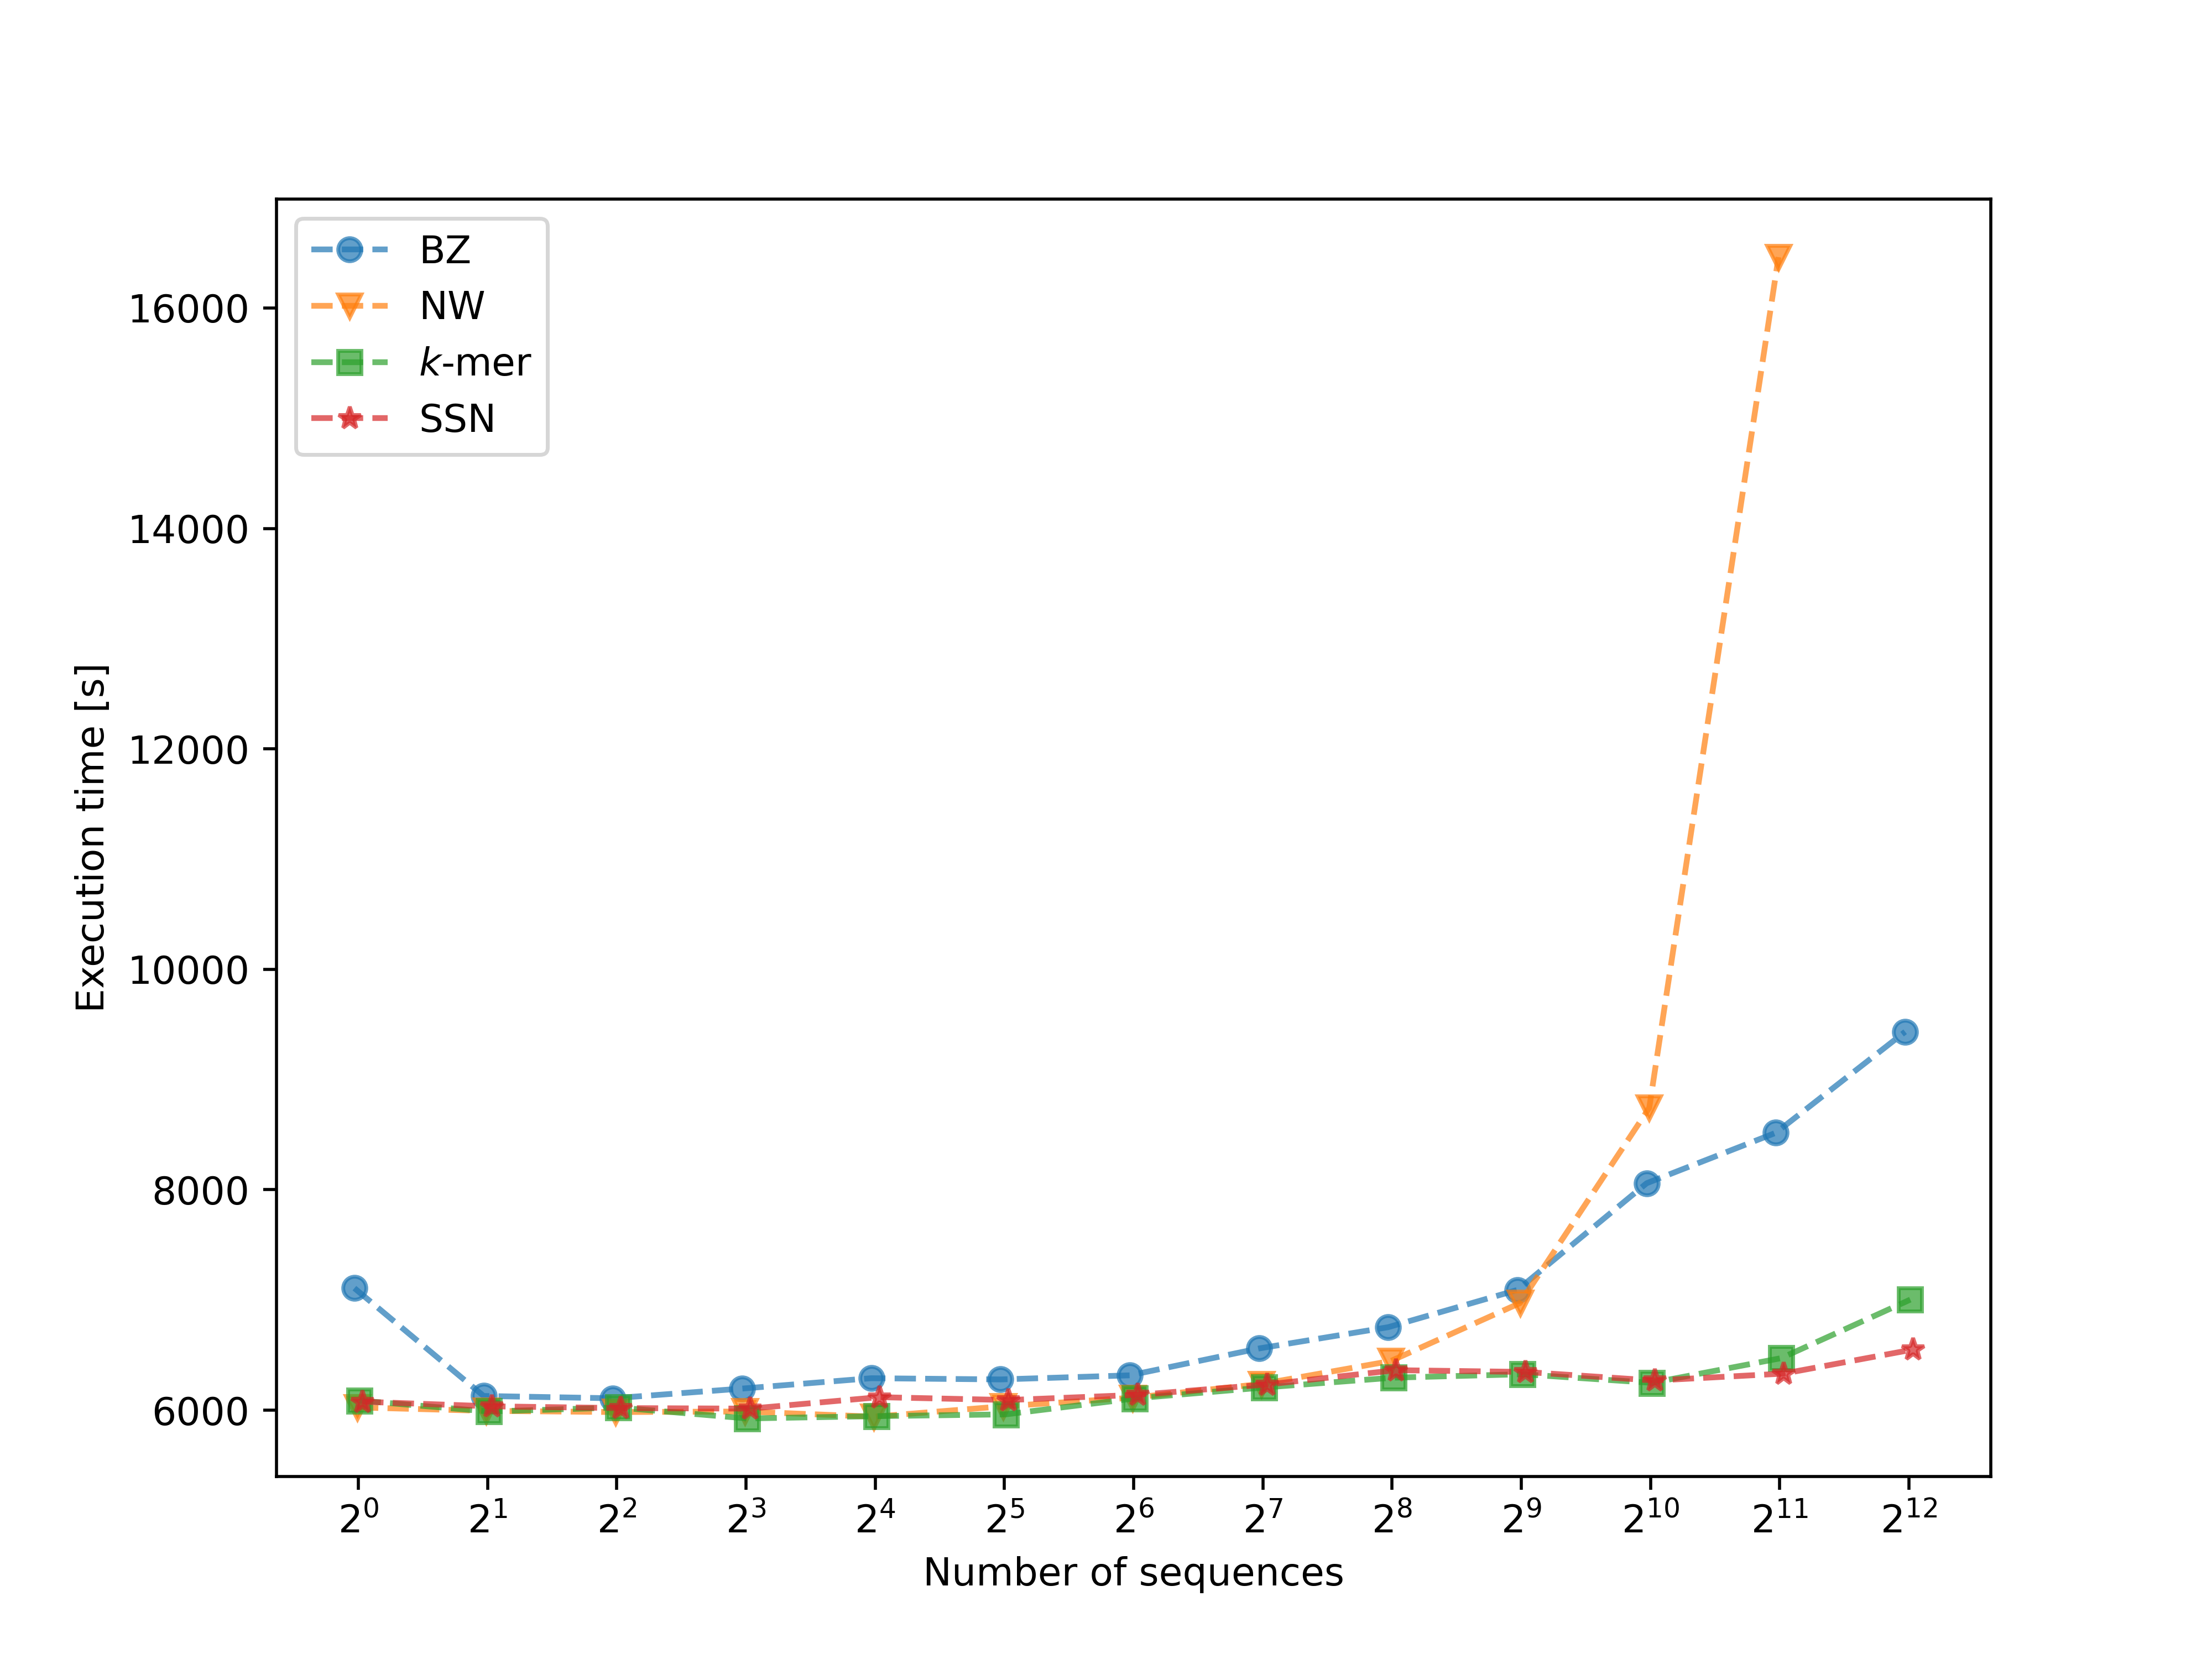
\includegraphics[width=\textwidth]{pictures/experiment_duration.png}
                    \end{center}
                    \caption{
                        Taxonomic classification execution time.
                    }\label{Picture:Experiment:Duration}
                \end{figure}

                \begin{table}\centering
                    \caption{Taxonomic classification execution time.}\label{Table:Experiment:Duration}
                    \begin{tabularx}{\textwidth}{|c||R|R|R|R|}
                        \hline
                        \multirow{2}{*}{\textbf{Number of sequences}} & \multicolumn{4}{|c|}{\textbf{Execution time [s]}} \\ \cline{2-5}
                                        & \textbf{NP} & \textbf{NW} & \textbf{$k$-mer} & \textbf{ANN} \\ \hline \hline
                                        1 & 7107 & \textbf{6025} & 6087 & 6077\\ \hline
                                        2 & 6129 & 5994 & \textbf{5988} & 6035\\ \hline
                                        4 & 6108 & \textbf{5983} & 6024 & 6019\\ \hline
                                        8 & 6196 & 5988 & \textbf{5925} & 6014\\ \hline
                                        16 & 6290 & \textbf{5941} & 5946 & 6118\\ \hline
                                        32 & 6279 & 6035 & \textbf{5962} & 6092\\ \hline
                                        64 & 6316 & 6113 & \textbf{6107} & 6139\\ \hline
                                        128 & 6560 & 6238 & \textbf{6206} & 6233\\ \hline
                                        256 & 6753 & 6446 & \textbf{6295} & 6363\\ \hline
                                        512 & 7091 & 6972 & \textbf{6326} & 6347\\ \hline
                                        1024 & 8059 & 8743 & \textbf{6248} & 6269\\ \hline
                                        2048 & 8517 & 16461 & 6472 & \textbf{6332}\\ \hline
                                        4096 & 9433 & \textbf{-1} & 7003 & 6550\\ \hline

                    \end{tabularx}
                \end{table}

                \paragraph{Conclusions}
                The method using the modified Needleman-Wunsch algorithm exhibited the fastest increase in execution time for taxonomic classification. The sharp rise is due to the time-consuming process of comparing sequences with each other. Despite reducing the number of sequences being classified, the execution time using this method exceeded that of taxonomic classification for all sequences.

                The methods using $k$-mer embeddings and ANNs showed comparable execution times, with a slight advantage for the former. Both methods use sequence representations for comparison, resulting in a slower increase in the time needed to build the dissimilarity matrix. These methods performed faster than taxonomic classification for all sequences. In the case of the ANN, the shorter execution time for $4096$ sequences could be due to the simultaneous computation of embeddings for all sequences using the GPU.

            \subsubsection{Experiment 2: Taxonomic classification quality}

                \paragraph{Objective}
                Examining the quality of taxonomic classification using the implemented methods in comparison to the taxonomic classification of all sequences.

                \paragraph{Assumptions}
                \begin{enumerate}
                    \item {
                        Sequences clustering is deterministic.
                    }
                    \item {
                        \texttt{BLASTn} is deterministic and always returns the same results for a given sequence and specified parameters.
                    }
                    \item {
                        In the case where it is not possible to compute the quality for a given taxonomic classification run, a quality value of $0$ is assumed. This value is not considered when calculating the weighted average quality.
                    }
                \end{enumerate}

                \paragraph{Results}
                The quality of the classification was calculated using the measure expressed by equation~\ref{Equation:Quality} for the implemented methods in comparison to the full taxonomic classification. Figure~\ref{Picture:Experiment:Quality} shows a graph of classification quality as a function of the number of input sequences, with detailed quality results provided in Table~\ref{Table:Experiment:Quality}. The weighted average quality calculated using equation~\ref{Equation:WeightedAverageQuality} for the method with the modified Needleman-Wunsch algorithm was $0.899$, for the $k$-mer embedding method it was $0.921$, and for the method using the artificial neural network, it was $0.944$.

                \begin{figure}[!htb]
                    \begin{center}
                        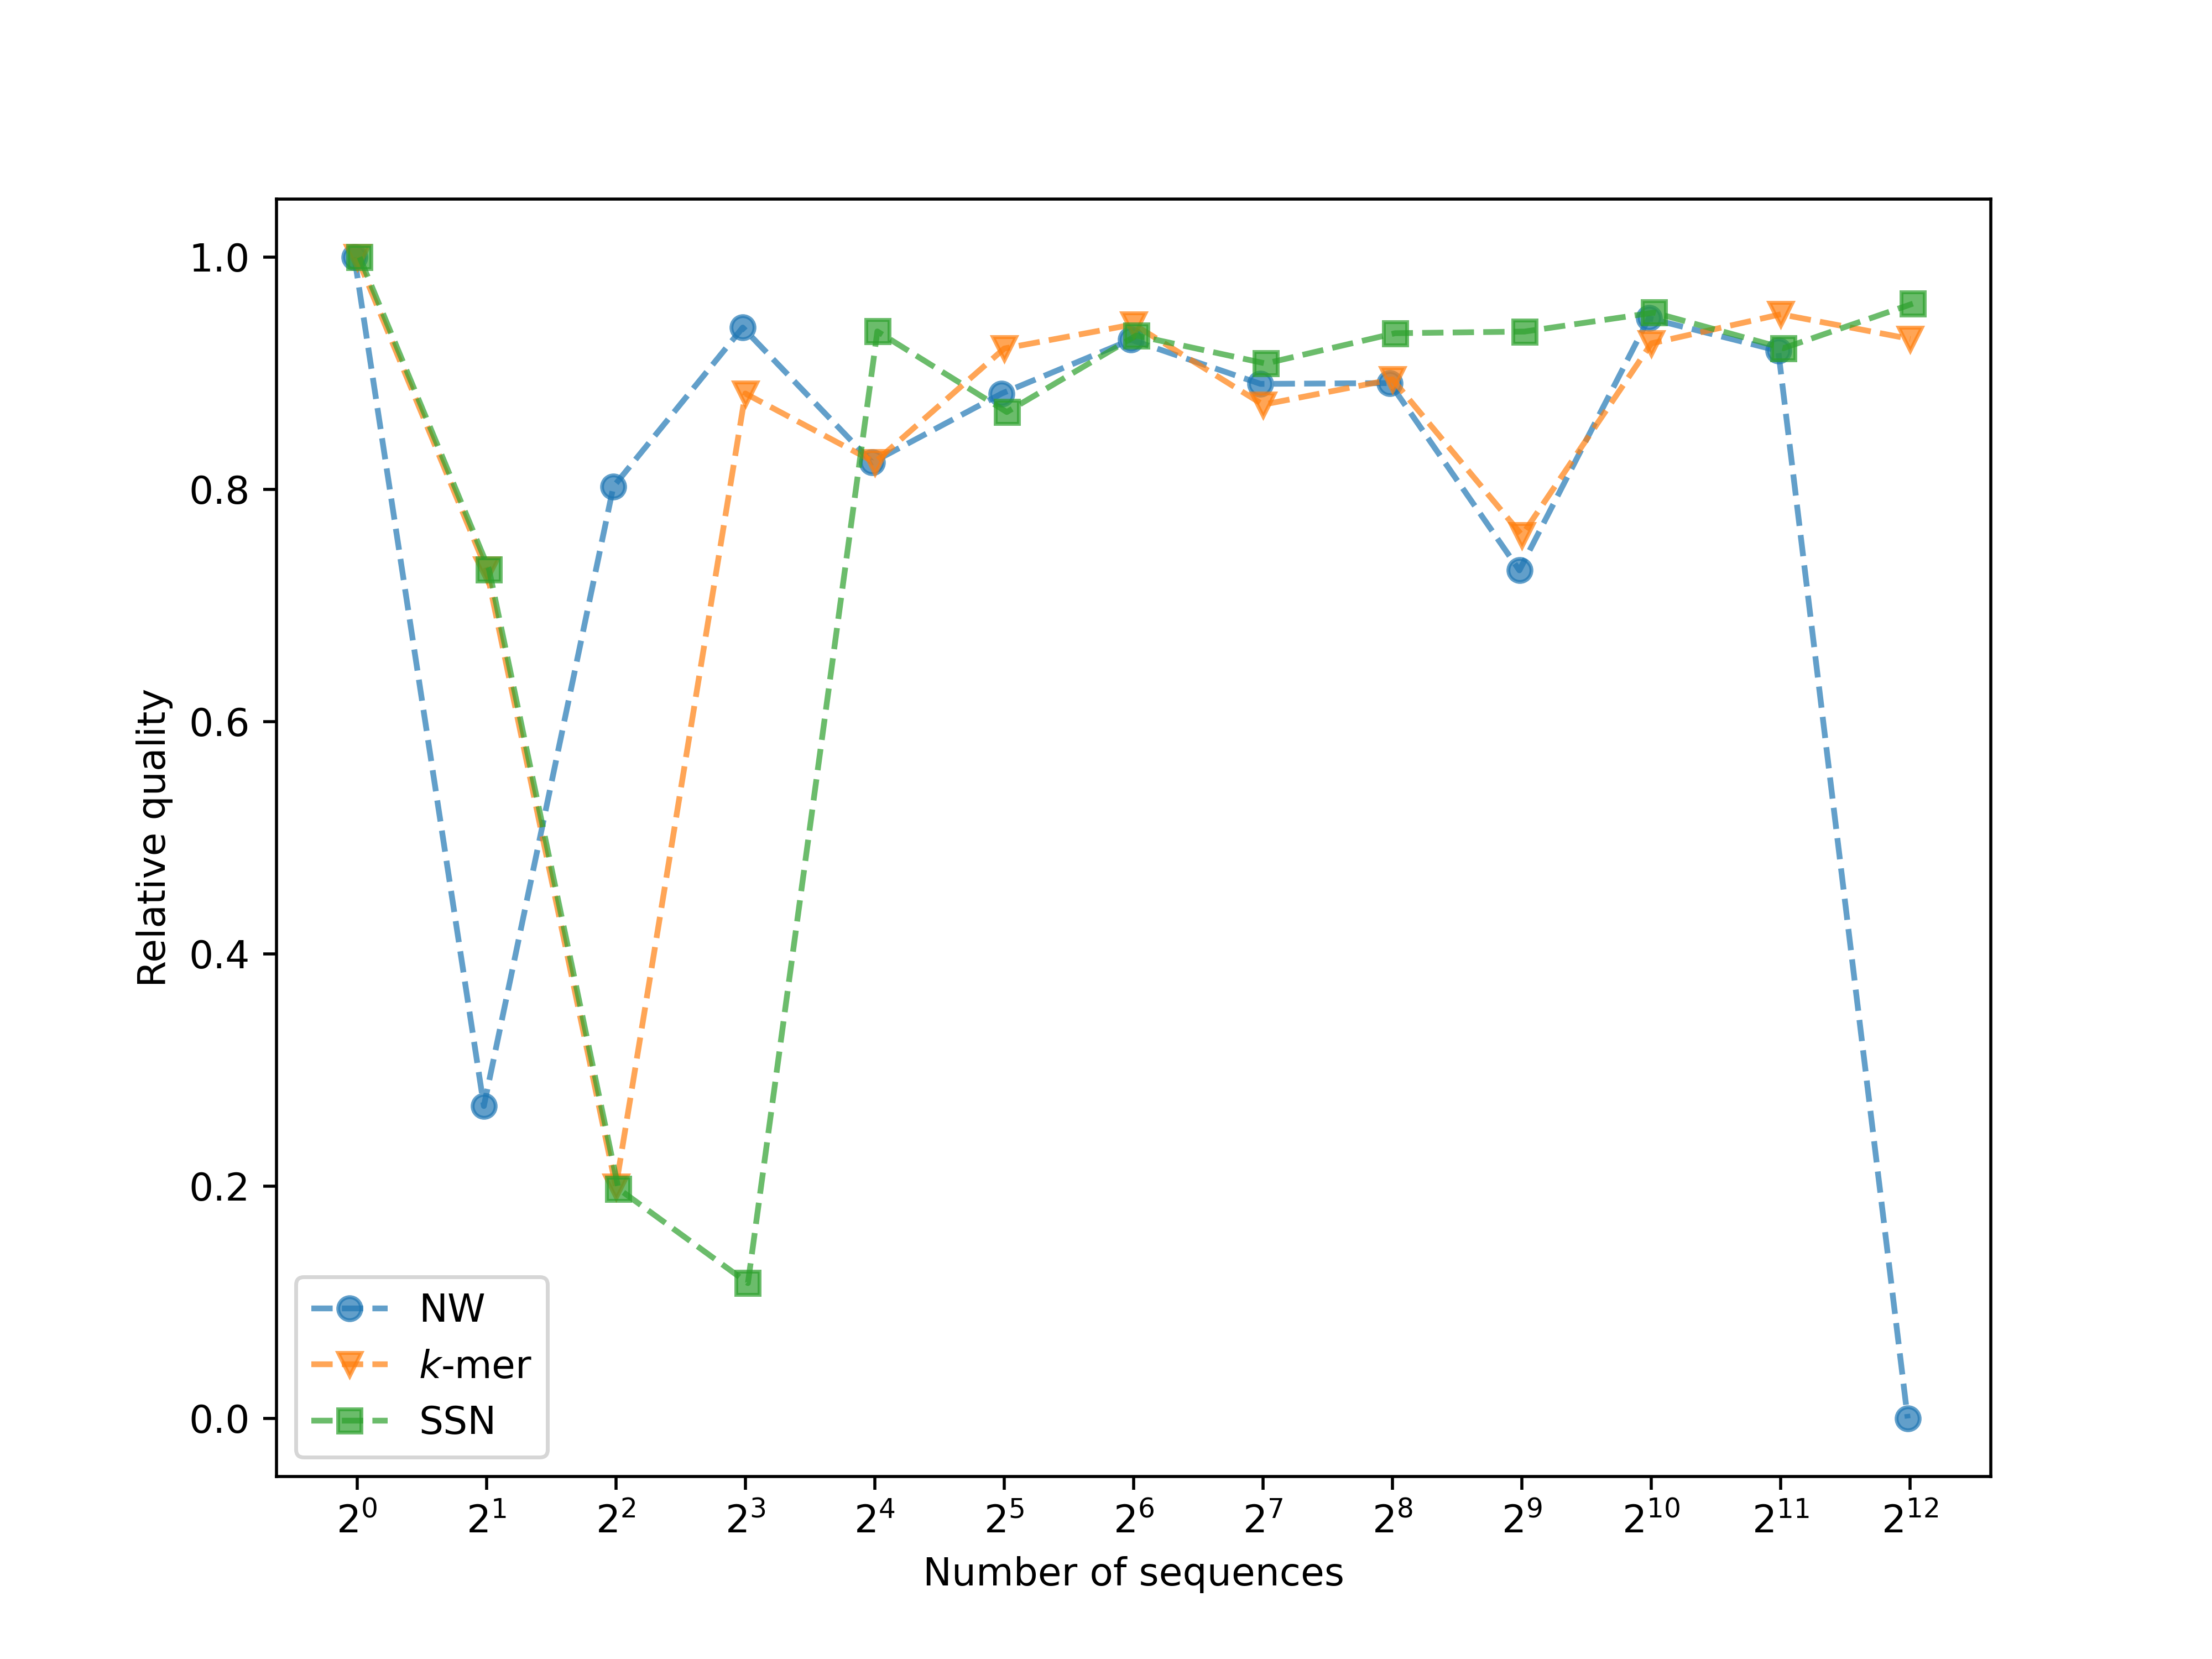
\includegraphics[width=\textwidth]{pictures/experiment_quality.png}
                    \end{center}
                    \caption{
                        Taxonomic classification quality.
                    }\label{Picture:Experiment:Quality}
                \end{figure}

                \begin{table}\centering
                    \caption{Taxonomic classification quality.}\label{Table:Experiment:Quality}

                    \begin{tabularx}{\textwidth}{|c|R|R|R|}
                        \hline
                        \multirow{2}{*}{\textbf{Number of sequences}} & \multicolumn{3}{|c|}{\textbf{Method}} \\ \cline{2-4}
                        & \textbf{NW} & \textbf{$k$-mer} & \textbf{ANN} \\ \hline \hline
                        1 & \textbf{1.0} & \textbf{1.0} & \textbf{1.0}\\ \hline
                        2 & 0.27 & \textbf{0.73} & \textbf{0.73}\\ \hline
                        4 & \textbf{0.8} & 0.2 & 0.2\\ \hline
                        8 & \textbf{0.94} & 0.88 & 0.12\\ \hline
                        16 & 0.82 & 0.82 & \textbf{0.94}\\ \hline
                        32 & 0.88 & \textbf{0.92} & 0.87\\ \hline
                        64 & 0.93 & \textbf{0.94} & 0.93\\ \hline
                        128 & 0.89 & 0.87 & \textbf{0.91}\\ \hline
                        256 & 0.89 & 0.89 & \textbf{0.93}\\ \hline
                        512 & 0.73 & 0.76 & \textbf{0.94}\\ \hline
                        1024 & \textbf{0.95} & 0.93 & \textbf{0.95}\\ \hline
                        2048 & 0.92 & \textbf{0.95} & 0.92\\ \hline
                        4096 & 0.0 & 0.93 & \textbf{0.96}\\ \hline
                    \end{tabularx}
                \end{table}

                \paragraph{Conclusions}
                All implemented methods achieved very good classification quality results, exceeding $0.7$ in cases where the number of groups was significantly larger than the number of input sequences. The weighted average quality for all methods also reached a high value.

                The method using the artificial neural network achieved the best weighted average quality, slightly outperforming the $k$-mer embedding method and the method with the modified Needleman-Wunsch algorithm. The artificial neural network method owes its result to the model's consideration of the full sequence structure, which allowed for a better determination of dissimilarity between sequences.

    \clearpage
    \section{Discussion}

        \subsection{Interpretation of Results}

            The results of the experiments partially confirmed the expectations set at the beginning of the research. All methods achieved satisfactory taxonomic classification quality. The method utilizing the artificial neural network performed particularly well, achieving the best weighted average classification quality while maintaining execution time comparable to the method based on $k$-mer embeddings. The low taxonomic classification quality with a small number of input sequences may be due to the inappropriate selection of group representatives, caused by too few available sequences. Therefore, the implemented methods should only be used in cases where the number of input sequences exceeds a certain threshold, and their use significantly reduces the time required for the taxonomic classification process. For the data tested, this condition is met for $128$ sequences, where the taxonomic classification quality was no less than $0.87$, and the use of any grouping method reduced the time by at least 5 minutes, resulting in a $5\%$ acceleration compared to the taxonomic classification of all sequences. The use of the artificial neural network allowed for an improvement in classification quality compared to other methods. In addition to achieving good classification quality, it does not lag behind classical methods.

        \subsection{Limitations}

            \subsubsection{Experiments Duration}
                The full process of taxonomic classification of DNA sequences for each method and each experimental subset took approximately 5 days, which led to the limitation of the number of number of experiments to single run and subset size to $4096$ sequences.

            \subsubsection{Single Dataset}  
                In work, only one sample from the chosen dataset was used. The selection of a sample containing DNA sequences from the human skin microbiome might have limited the space of analyzed sequences, which could have influenced the experimental results, as the both the artificial neural network and the experiments used DNA sequences from the same microbiome.

            \subsubsection{Single Dissimilarity Matrix}
                The use of a single dissimilarity matrix for all sequences limits the number of input sequences, as the matrix build time of matrix scales quadratically with the number of sequences.

        \subsection{Possible Improvements}

            \subsubsection{Architecture of Artificial Neural Network}

                The proposed artificial neural network architecture is not flexible and is only suitable for analyzing sequences of similar lengths. It would be possible to modify the model's architecture to incorporate recurrent neural networks (RNNs) and transformers, enabling the processing of sequences with varying lengths. RNNs and transformers could replace the first part of the model, which currently relies on convolutional layers. They would be used to create embeddings, which would later be processed by linear layers to generate an embedding that preserves dissimilarity properties.

            \subsubsection{Batching sequences}

                Creating a single dissimilarity matrix for very large samples is not optimal, as it significantly impacts the performance of the method. To address this issue, pre-clustering the sequences into batches can provide a solution. Processing in batches may reduce quality but allows for maintaining a short execution time.

            \subsubsection{Automatated Determination Of The Number of Groups}

                Current approach takes the number of created groups as a parameter, which can influence the quality of the results. For very similar sequences, a large number of groups is excessive and does not improve the results. Conversely, for highly diverse sequences, a low number of groups can reduce quality. Automating the determination of the optimal number of grousp could solve the issue and minimize the need for fine-tuning 

    \clearpage
    \section{Conclusions and Future Work}

        \subsection{Summary of Findings}

            \temporary{
                Stworzone rozwiązanie zostało zaimplementowane przy użyciu języka Rust, a jego struktura została odpowiednio zorganizowana w moduły, które realizują poszczególne funkcjonalności i umożliwiają łatwe rozszerzanie aplikacji. Aplikacja konsolowa pozwala w bardzo prosty sposób na uruchomienie procesu analizy oraz ustawienie wszystkich parametrów dostępnych dla zaimplementowanych metod. Aplikacja przeglądarkowa umożliwia uruchomienie analizy przy użyciu najlepszego zestawu parametrów oraz wyświetlenie wyników w czytelnej dla użytkownika postaci.

                Przeprowadzone eksperymenty wykazały, że nowa metoda oparta na sztucznych sieciach neuronowych pozwala na osiągnięcie wyższej jakości od metod klasycznych, jednocześnie zachowując czas wykonania porównywalny z metodą klasyczną wykorzystującą $k$-mery.
            }

        \subsection{Future Research Directions}

            \temporary{
                \subsubsection{Narzędzie do klasyfikacji taksonomicznej oparte o model sztucznej sieci neuronowej}

                Narzędzia do klasyfikacji taksonomicznej w większości opierają się na obliczaniu podobieństwa między sekwencjami wejściowymi a sekwencjami znajdującymi się w bazie danych sekwencji w celu znalezienia sekwencji, które są podobne. Wykorzystane w eksperymentach narzędzie \texttt{BLASTn} wykorzystuje $k$-mery do określenia podobieństwa między sekwencjami. 
                Grupowanie sekwencji, które zostało wykorzystane w pracy, wykonuje podobne operacje, do tych, które są wykonywane przez narzędzia do klasyfikacji taksonomicznej. Możliwe byłoby zatem stworzenie własnego narzędzia, które wykorzystywałoby bezpośrednio model sztucznej sieci neuronowej do określenia podobieństwa między sekwencjami i klasyfikacji taksonomicznej. Wykorzystanie sztucznych sieci neuronowych w przypadku wydajnej implementacji mogłoby pozwolić na osiągnięcie akceptowalnego czasu działania przy wyższej jakości.
            }

\end{document}